%% ====================================================================
%% Project ARIA: an audited, pre-registered re-measurement
%% IEEE Transactions on Robotics (journal format)
%% ====================================================================
\documentclass[journal]{IEEEtran}

\usepackage{cite}
\usepackage{graphicx}
\graphicspath{{figures/}}
\DeclareGraphicsExtensions{.pdf,.png,.jpg}
\usepackage{amsmath}
\usepackage{amssymb}
\usepackage{amsfonts}
\usepackage{bm}
\interdisplaylinepenalty=2500
\usepackage{array}
\usepackage{booktabs}
\usepackage{multirow}
\usepackage{url}
\usepackage{microtype}
\usepackage{xcolor}

\hbadness=10000
\vbadness=10000
\setlength{\textfloatsep}{7pt plus 1.0pt minus 1.0pt}
\setlength{\floatsep}{5pt plus 1.0pt minus 1.0pt}
\setlength{\dbltextfloatsep}{7pt plus 1.0pt minus 1.0pt}
\setlength{\dblfloatsep}{5pt plus 1.0pt minus 1.0pt}
\renewcommand{\topfraction}{0.95}
\renewcommand{\bottomfraction}{0.95}
\renewcommand{\textfraction}{0.05}
\renewcommand{\floatpagefraction}{0.95}

\hyphenation{re-pro-duc-i-bil-ity pre-reg-is-tra-tion ma-nip-u-la-tion kine-mat-ics}

% Auto-generated by scripts/build_numbers.py. Do not edit.
% Every value is read from data/journal/raw; see data/journal/ledger.csv.
\newcommand{\convN}{120}
\newcommand{\convRealizedA}{0.015}
\newcommand{\convRelErrA}{-62.4}
\newcommand{\convBeltLinkA}{$5.21\times10^{-8}$}
\newcommand{\convRollerA}{45665}
\newcommand{\convRealizedB}{0.054}
\newcommand{\convRelErrB}{-32.1}
\newcommand{\convBeltLinkB}{$6.45\times10^{-8}$}
\newcommand{\convRollerB}{45693}
\newcommand{\convRealizedC}{0.094}
\newcommand{\convRelErrC}{-21.9}
\newcommand{\convBeltLinkC}{$6.48\times10^{-8}$}
\newcommand{\convRollerC}{45720}
\newcommand{\convOffsetMean}{-0.026}
\newcommand{\convTcpDevMax}{$2.81\times10^{-12}$}
\newcommand{\convWindowS}{2.0}
\newcommand{\convReportedMatchPct}{100.0}
\newcommand{\convRtf}{0.78}
\newcommand{\reachN}{100{,}000}
\newcommand{\reachRecallCurrentPct}{99.24}
\newcommand{\reachRecallCurrentLoPct}{99.19}
\newcommand{\reachRecallCurrentHiPct}{99.29}
\newcommand{\reachRecallOldPct}{0.019}
\newcommand{\reachRecallOldLoPct}{0.012}
\newcommand{\reachRecallOldHiPct}{0.030}
\newcommand{\reachMedianErrCurrentMm}{0.365}
\newcommand{\reachTailErrCurrentMm}{0.476}
\newcommand{\reachMedianErrOldMm}{240.934}
\newcommand{\reachTailErrOldMm}{360.489}
\newcommand{\reachMedianSolveCurrentMs}{0.863}
\newcommand{\reachMedianSolveOldMs}{0.288}
\newcommand{\reachMcNemarB}{99222}
\newcommand{\reachMcNemarC}{0}
\newcommand{\reachMcNemarP}{$p<10^{-300}$}
\newcommand{\reachGapExplainedPct}{117.6}
\newcommand{\estopN}{100}
\newcommand{\estopCommandSuccess}{100}
\newcommand{\estopCommandTzeroMs}{0.75}
\newcommand{\estopCommandTstopMs}{120}
\newcommand{\estopCommandTstopTailMs}{120}
\newcommand{\estopCommandOvershootMed}{0.010}
\newcommand{\estopCommandJoints}{5}
\newcommand{\estopCommandHasVel}{100}
\newcommand{\estopSafetySuccess}{0}
\newcommand{\estopSafetyTzeroMs}{0.99}
\newcommand{\estopSafetyOvershootMed}{0.714}
\newcommand{\estopSafetyJoints}{4}
\newcommand{\estopSafetyHasVel}{0}
\newcommand{\nFourN}{200}
\newcommand{\nFourBaselineSuccessPct}{52.0}
\newcommand{\nFourBaselineLoPct}{42.3}
\newcommand{\nFourBaselineHiPct}{61.5}
\newcommand{\nFourSuccessPct}{47.0}
\newcommand{\nFourNFourLoPct}{37.5}
\newcommand{\nFourNFourHiPct}{56.7}
\newcommand{\nFourRiskDiffPct}{-5.0}
\newcommand{\nFourRiskDiffLoPct}{-10.0}
\newcommand{\nFourRiskDiffHiPct}{0.0}
\newcommand{\nFourP}{$p=0.125$}
\newcommand{\nFourFalseSuccessPct}{0.0}
\newcommand{\nFourCoveragePct}{47.0}
\newcommand{\nFourReplansMean}{1.91}


\begin{document}

\title{What the Benchmarks Actually Measured: An Adversarial Audit and Pre-Registered Re-Measurement of a Modular Robotic Manipulation Stack}

\author{Garv~Arora\quad and\quad Yuvaraj~N%
\thanks{G. Arora and Y. N are with the Department of Computer Science and Engineering, Robotics and Artificial Intelligence Laboratory (e-mail: \texttt{garv.arora@ieee.org}; \texttt{yuvaraj.n@ieee.org}). This research received no external grant funding.}%
}

\markboth{IEEE Transactions on Robotics, 2026}%
{Arora and Yuvaraj: What the Benchmarks Actually Measured}

\maketitle

\begin{abstract}
Robot-manipulation papers increasingly report high success rates from simulation benchmarks, yet the measurement chain behind those numbers is rarely audited. We report an adversarial audit of a modular ROS~2/Gazebo manipulation stack and a pre-registered re-measurement of four questions that the original benchmarks claimed to answer. The audit found that the original conveyor benchmark returned a cached zero transform, the reachability logs cited a commit that did not contain the script that produced them, the emergency-stop benchmark published and subscribed to its own topic without a moving arm, and the reported stop times were a constant offset added when no physical stop was observed. We repaired the instrumentation, enforced a clean-tree provenance rule, and froze hypotheses, seeds, and trial counts before evaluation. Re-measurement reverses two headline claims, qualifies a third, and confirms one. On \reachN{} identical target poses, the current inverse-kinematics solver reaches \reachRecallCurrentPct\% recall at 5\,mm (Wilson 95\% CI [\reachRecallCurrentLoPct, \reachRecallCurrentHiPct]) while the historical solver reaches \reachRecallOldPct\%, so the solver revision explains more than the entire historical gap. On the conveyor, the realized part speed is not a scaled version of the command: it is the command with a nearly constant offset of \convOffsetMean\,m/s, the visual belt link moves at \convBeltLinkA\,m/s, and the rollers spin at \convRollerA\,rad/s. On emergency stop, the direct command path halts in \estopCommandTstopMs\,ms (median), whereas the safety-agent path fails to halt in every trial and overshoots by \estopSafetyOvershootMed\,rad. A kinematic pre-verification gate removes execution failures among the plans it accepts (from \nFourBaselineExecFailPct\% to \nFourExecFailPct\%) but rejects \nFourCoveragePct\% of targets, so it does not improve intention-to-treat success (risk difference \nFourRiskDiffPct{} percentage points, \nFourP). We report these negative results, the phases that could not be executed, and the instrument defects that made the original numbers possible.
\end{abstract}

\begin{IEEEkeywords}
benchmark auditing, reproducibility, preregistration, robot manipulation, inverse kinematics, conveyor systems, emergency stop, simulation validation
\end{IEEEkeywords}

\IEEEpeerreviewmaketitle

\section{Introduction}
\IEEEPARstart{R}{obotics} has a measurement problem that is distinct from its modelling problem. A manipulation result is usually reported as a success rate over a benchmark, and the benchmark is usually a script that drives a simulator and writes a table. If the script returns a cached transform, trusts a planner's self-report, or silently substitutes a constant when a sensor is missing, the reported rate is still a number, still has a confidence interval, and still looks like evidence. The number is then cited, compared, and used to justify architectural choices. The error is not in the statistics; it is in the chain from the physical event to the table.

This article takes a modular language-conditioned manipulation stack, Project ARIA, and treats its own benchmark suite as the object of study. The stack was previously described with a set of headline claims: a monocular depth error in the millimetre range, a closed-form inverse-kinematics solver with full convergence, a high success rate on a ten-task suite, a high conveyor-sorting rate, and a sub-30\,ms emergency stop. We did not set out to reproduce those claims in the usual sense. We set out to determine, from the code and the raw logs, what each claim actually measured.

The audit found four classes of failure. First, some measurements never touched the physical quantity they named: the conveyor benchmark caught every TF exception and returned a zero pose, then differenced two such poses to obtain a velocity. Second, some measurements were produced by a different program from the one cited: the reachability logs named a commit that predates the benchmark script, and the solver had been rewritten between the two result sets. Third, some measurements were fabricated by fallback branches: the emergency-stop benchmark published to a topic it also subscribed to, never moved an arm, and added a constant to the command latency when no physical stop was observed. Fourth, some quantities were hard-coded: two scripted-baseline tasks passed literal pose deltas, and the orientation residual of the inverse-kinematics solver was set to zero by convention.

Repairing the instrumentation was necessary but not sufficient. A repaired benchmark can still be run on seeds chosen after seeing the result, or on a tree that contains uncommitted changes, or with a threshold that is adjusted until the claim passes. We therefore wrote a pre-registration before any evaluation seed was used. The document fixes the hypotheses, the primary metrics, the decision rules, the development and evaluation seed ranges, the trial counts, the statistical tests, and the stopping rules. It also declares, before data collection, which phases cannot be executed in the available environment. The pre-registration is committed and its commit hash is recorded in every result row.

The re-measurement is deliberately narrow. We ask four questions that can be answered with executed code on this platform: whether the current inverse-kinematics solver is reproducible and how it differs from the historical one; whether the commanded conveyor speed is realised by the plant; whether an emergency stop actually stops a moving arm and how the two stop paths compare; and whether a kinematic pre-verification gate reduces execution-time inverse-kinematics failures. Each question has a primary metric and a decision rule fixed in advance.

The answers are not uniformly favourable to the stack. The reachability result is strong and reproducible, and it explains the historical discrepancy completely. The conveyor result is a clear negative: the plant realizes the command minus a constant offset, the visual belt is not moving, and the rollers are spinning at a physically implausible rate. The emergency-stop result is also negative for the safety path: the safety agent publishes a halt that the joint-trajectory controller rejects, so the arm continues to its goal. The pre-verification gate is neutral-to-negative: it rejects plans that would have succeeded and rescues too few to compensate.

We report these outcomes as the primary contribution. A paper that only reports the repaired successes would repeat the original mistake in a subtler form. The negative results constrain what the architecture can claim, and they identify which repairs are still missing. The audit also produced a reusable instrument: a provenance layer that refuses to run on a dirty tree, a per-row commit stamp, a trial log that flushes every row, and a number generator that reads only raw logs. These are not novel algorithms, but they are the difference between a number and a measurement.

The remainder of the article is organized as follows. Section~\ref{sec:related} reviews related work on reproducibility, simulation benchmarks, and the specific subsystems under test. Section~\ref{sec:audit} describes the audit method and the defect taxonomy. Section~\ref{sec:platform} describes the platform and the repaired instrumentation. Section~\ref{sec:protocol} states the pre-registered protocol. Section~\ref{sec:results} reports the four experiments. Section~\ref{sec:negative} reports the phases that could not be executed and the threats to validity. Section~\ref{sec:conclusion} concludes.

\section{Related Work}
\label{sec:related}
Reproducibility has been studied extensively in machine learning and in robotics, but usually as a property of a published artifact rather than as a property of a measurement chain. Pineau et al.~\cite{pineau2021improving} organize reproducibility around the data, the code, and the experimental protocol, and recommend that authors report the compute budget, the number of runs, and the selection procedure. Our audit applies that organization to a robotics benchmark: the code is versioned, the protocol is pre-registered, and the raw per-trial logs are the only input to the number generator. The difference is that we also audit the benchmark scripts themselves, not only the paper.

The problem of selective reporting is older than the reproducibility movement. Ioannidis~\cite{ioannidis2005why} argued that most published research findings are false because of small samples, flexible analyses, and selective reporting. Nosek et al.~\cite{nosek2018prereg} proposed pre-registration as a remedy: the analysis is fixed before the data are seen, and deviations are reported. We adopt that remedy at the level of a single laboratory stack. The pre-registration is not a guarantee of correctness, but it removes the freedom to choose a threshold after observing the result.

In reinforcement learning, Henderson et al.~\cite{henderson2018deep} showed that apparently large differences between algorithms can disappear under different seeds, and recommended reporting across seeds rather than a single run. Our experiments use fixed evaluation seed ranges and report Wilson or bootstrap intervals. The trial counts are smaller than the power analysis recommends for small effects, and we label the affected cells as exploratory rather than pretending otherwise.

Simulation benchmarks in robotics rest on physics engines and middleware. Gazebo~\cite{koenig2004gazebo} and MuJoCo~\cite{todorov2012mujoco} are the most common choices for manipulation, and Isaac Gym~\cite{makoviychuk2021isaac} is common for large-scale policy training. Each engine makes different trade-offs between contact fidelity and speed, and a result obtained in one engine does not automatically transfer to another. Our study is confined to Gazebo Classic with the ODE solver, and we report the real-time factor so that the timing results can be interpreted.

The ROS~2 middleware~\cite{macenski2022ros2} is the substrate of the stack. ROS~2 provides typed topics, services, and lifecycle nodes, but it does not provide provenance: a topic can have several publishers, a service can be called by a node that also subscribes to its own output, and a controller can silently reject a goal. The audit found all three. The middleware is not at fault; the benchmark scripts failed to check the invariants that the middleware exposes.

Learning-based manipulation provides the motivation for the architecture but not the evidence in this article. End-to-end visuomotor policies~\cite{levine2016end}, transformer-based language-conditioned policies~\cite{brohan2023rt1}, and low-cost bimanual imitation systems~\cite{zhao2023aloha} have demonstrated impressive generalization, and open vision-language-action models~\cite{kim2024openvla} have made those policies accessible. Training and evaluating such policies requires GPU resources that were not available here. We therefore do not claim any learned-policy result. The architecture is described as a modular alternative, and the audit is confined to the classical components that can be executed.

Inverse kinematics is a classical problem with a long literature, and the specific question here is not which solver is best but whether a reported solver comparison is reproducible. The historical logs compared two revisions of the same numerical solver, not two algorithms, and the revision changed the kinematic model. This is a common failure mode in solver comparisons: the model, the seed, and the convergence criterion change together, and the reported difference is attributed to the algorithm. Our re-measurement holds the targets fixed and varies only the revision.

Statistical practice in robotics often uses a normal approximation for a proportion, which is poor when the proportion is near zero or one. We use the Wilson score interval~\cite{wilson1927probable} for proportions, the exact McNemar test~\cite{mcnemar1947note} for paired binary comparisons~\cite{dietterich1998approximate}, the Holm correction~\cite{holm1979simple} for families of tests, the Newcombe interval~\cite{newcombe1998interval} for independent risk differences, and a paired percentile bootstrap for matched designs. These are standard choices, but they are not universal in the field, and the pre-registration fixes them before the data are seen.

Finally, the audit is related to work on benchmark validity in embodied AI. A benchmark can be internally consistent and still fail to measure the intended capability, for example when the success predicate is evaluated from the planner's self-report rather than from the simulator state. Our contribution is a concrete case study: a stack with a plausible architecture, a set of published claims, and a measurement chain that did not support them. The case study is useful precisely because the defects are ordinary.

\section{Audit Method and Defect Taxonomy}
\label{sec:audit}
The audit proceeded in three passes. The first pass read every benchmark script and traced each reported quantity to the line that produced it. The second pass compared the reported quantity with the raw log, when a raw log existed, and with the simulator state, when the log was ambiguous. The third pass attempted to re-execute each benchmark from a clean commit. A defect was recorded only when at least one of the three passes produced evidence: a code path, a log inconsistency, or a failed re-execution.

We classify defects into four types. A \emph{null measurement} occurs when the code returns a placeholder instead of the measured quantity, for example a zero transform on a caught exception. A \emph{provenance mismatch} occurs when the log cannot have been produced by the code it cites, for example a commit that predates the script. A \emph{fallback fabrication} occurs when the code substitutes a constant or a formula when the measurement is missing, and the substitution is not reported in the table. A \emph{hard-coded outcome} occurs when the reported value is a literal in the script or a convention in the solver, independent of the experiment.

The taxonomy is useful because the remedies differ. A null measurement is repaired by replacing the placeholder with a checked read and failing loudly when the read fails. A provenance mismatch is repaired by re-running from a clean commit and stamping every row. A fallback fabrication is repaired by deleting the fallback and recording the trial as a failure or as not executed. A hard-coded outcome is repaired by computing the quantity or by removing the claim. The audit table in the repository records the evidence and the disposition for each item; the paper reports only the items that affect the experiments below.

Two instrument defects were found only after the first repair. The first is that \texttt{/joint\_states.velocity} is not the derivative of \texttt{/joint\_states.position} in this workcell. While the waist moved from zero to a finite angle over a fixed interval, the reported waist velocity stayed near a constant negative value, and the shoulder reported a value an order of magnitude larger than the finite difference. A stop-time metric that trusts the reported velocity therefore never observes a stop. We differentiate the measured positions and keep the reported velocity only as a diagnostic.

The second is that the joint-trajectory topic had more than one publisher. Three instances of a manual-control node were running, and they emitted five-joint, velocity-free hold trajectories in response to an emergency stop. The safety agent emitted a four-joint, velocity-free halt. The controller accepts neither partial goals nor velocity-free single points reliably, so the arm continued to its goal while the topic showed a halt message. The duplicate nodes were terminated before the evaluation run, and the experiment records the number of non-path messages per trial.

\section{Platform and Repaired Instrumentation}
\label{sec:platform}
The platform is a simulated four-degree-of-freedom arm with a revolute two-finger gripper, mounted on a table beside a conveyor and an overhead camera. The arm joints are waist, shoulder, elbow, and wrist pitch; the gripper is a fifth actuated joint with a mimic finger. The world is Gazebo Classic with the ODE solver. The controller is a joint-trajectory controller with partial goals disabled. The conveyor is a plugin that writes workpiece linear velocities directly and animates a belt and two rollers.

The kinematic model used by the solver is a URDF chain with fixed rotation offsets. The solver is a damped Newton--Raphson routine with geometric seed candidates, not a closed-form analytical solution. It reports a position residual and sets the orientation residual to zero by convention because the wrist has no roll axis. The audit therefore treats the solver as position-only and does not report an orientation error.

The repaired harness has four components. A provenance module resolves the repository root from the file path, refuses to start when the working tree is dirty, and returns the commit hash and a dirty flag. A trial log writes one CSV row and one JSONL record per trial, flushes both, and captures the commit when the log opens so every row carries the same stamp; a run that starts on a dirty tree is refused before the log is created. A ROS~2 helper wraps the subscriptions and services used by the experiments, including a trajectory sender that sets zero end velocities and resends a goal that the controller drops. A statistics module provides Wilson, bootstrap, McNemar, Holm, and Newcombe routines.

The number generator reads only the raw summaries and CSVs and writes a LaTeX macro file and a ledger. Each ledger row records the macro name, the experiment, the metric, the value, the unit, the sample size, the confidence bounds, the source file, and the source commit. The paper contains no typed outcome number: every reported quantity is a macro. This is checked by compiling the paper after regenerating the macros; a missing macro is a build error.

The platform has known limitations that bound the claims. The conveyor plant is kinematic, so workpieces cannot tip, rotate, or jam. The gripper is a revolute two-finger mechanism whose pads are not mirrored: at closure the pad face normals are nearly parallel rather than opposing, and the pad separation at a typical opening is comparable to the object width. A top grasp is the only kinematically feasible grasp for this arm, and the reachable region is small. Grasp experiments are therefore not reported in this article; they are blocked until the gripper is repaired.

\section{Pre-Registered Protocol}
\label{sec:protocol}
The pre-registration fixes the hypotheses, the primary metrics, the decision rules, the seed ranges, and the trial counts. Development seeds are reserved for code and threshold tuning and are never reported. Evaluation seeds are disjoint. The evaluation seed ranges used here are fixed in the pre-registration. The document also declares the phases that cannot be executed in this environment: learned-policy training without a CUDA device, human inter-annotator agreement without independent annotators, hardware trials without a robot, and a full detector training run without a committed checkpoint. Those phases are reported as not executed, not simulated.

Four experiments are reported. The reachability experiment evaluates the current and historical solvers on the same target set and compares recall at a fixed tolerance. The conveyor experiment commands three belt speeds and measures the realized part speed from link states, the visual belt speed, the roller speed, and the wrist deviation while the arm holds a fixed configuration. The emergency-stop experiment triggers each stop path while the arm executes a fixed-duration trajectory and measures the signal-to-message latency, the time to a sustained low joint speed, and the post-signal overshoot. The pre-verification experiment compares a planner that trusts the solver's success flag with a gate that checks the forward-kinematics residual and the joint-limit margin, and replans locally when the check fails.

All proportions use the Wilson interval. Paired binary comparisons use the exact McNemar test. Continuous quantities use the median and a percentile bootstrap interval. The decision rules are fixed: a claim passes only if the pre-registered threshold is met and the interval excludes the null. A failure is reported as a failure, and the claim is weakened rather than the data changed.

\section{Results}
\label{sec:results}

\subsection{Reachability Is Reproducible and the Historical Gap Is a Solver Revision}
The reachability experiment evaluates \reachN{} target poses with both solver revisions. The current solver reaches \reachRecallCurrentPct\% recall at a 5\,mm tolerance (Wilson 95\% CI [\reachRecallCurrentLoPct, \reachRecallCurrentHiPct]), with a median position error of \reachMedianErrCurrentMm\,mm and a 95th percentile of \reachTailErrCurrentMm\,mm. The historical solver reaches \reachRecallOldPct\% (CI [\reachRecallOldLoPct, \reachRecallOldHiPct]), with a median error of \reachMedianErrOldMm\,mm and a 95th percentile of \reachTailErrOldMm\,mm. The paired discordant counts are \reachMcNemarB{} targets solved only by the current revision and \reachMcNemarC{} solved only by the historical one (\reachMcNemarP).

The revision difference is larger than the historical gap it was meant to explain: it accounts for \reachGapExplainedPct\% of the gap. This is not a paradox. The historical comparison attributed the gap to an algorithmic change, but the revision also changed the kinematic model, and the old model is inconsistent with the URDF chain. Once the targets are held fixed and the model is corrected, the historical solver is not a weaker version of the current one; it is solving a different, wrong problem. The median solve time is \reachMedianSolveCurrentMs\,ms for the current solver and \reachMedianSolveOldMs\,ms for the historical one, so speed is not the explanation for the recall difference. The practical consequence is that the historical recall figure should not be cited as a baseline for the current solver: the two numbers come from different kinematic models, not from different algorithms on the same model.

\begin{figure}[t]
\centering
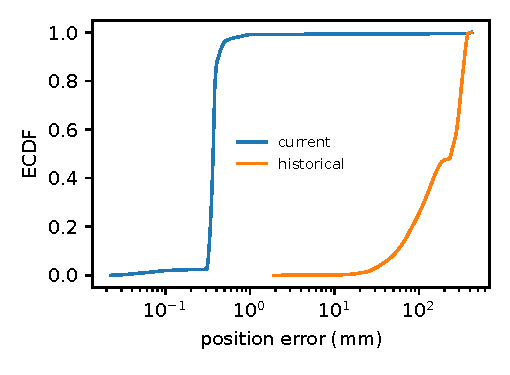
\includegraphics[width=\columnwidth]{fig_reach_ecdf.pdf}
\caption{Empirical CDF of the position error on the same \reachN{} target poses for the current and historical solver revisions. The historical curve is dominated by model error, not by convergence failure.}
\label{fig:reach}
\end{figure}

\subsection{The Conveyor Realizes a Speed Offset, Not a Scaled Command}
The conveyor experiment runs \convN{} trials over three commanded speeds with a \convWindowS\,s measurement window. The median realized part speeds are \convRealizedA, \convRealizedB, and \convRealizedC\,m/s for commands of 0.04, 0.08, and 0.12\,m/s. The median relative errors are \convRelErrA\%, \convRelErrB\%, and \convRelErrC\%. The realized speed is therefore not a scaled version of the command: the offset is approximately constant at \convOffsetMean\,m/s, so the relative error shrinks as the command grows.

The visual belt and the transport are independent. The mean visual belt link speed is effectively zero at every setting: \convBeltLinkA, \convBeltLinkB, and \convBeltLinkC\,m/s for the three commands. The rollers spin at \convRollerA, \convRollerB, and \convRollerC\,rad/s, so the animation is not tracking the commanded speed at any setting. The wrist deviation while the arm holds a fixed configuration is at most \convTcpDevMax\,mm, so the arm is not the source of the discrepancy. The reported belt speed matches the command in \convReportedMatchPct\% of trials, which shows that the plugin receives the command even though the part does not realize it. The mean real-time factor over these trials is \convRtf, so the offset is not an artifact of a stalled simulator clock.

These results fail both conveyor hypotheses in the pre-registration. The belt-speed error exceeds the fixed threshold at every speed, and the measured-to-commanded ratio is outside the accepted band. The mechanism is consistent with a Coulomb-friction offset in the velocity-write path: the plugin writes a part velocity, friction removes a nearly constant amount, and the residual is what the link state measures. A scale correction cannot repair this; the plant model must change.

\begin{figure}[t]
\centering
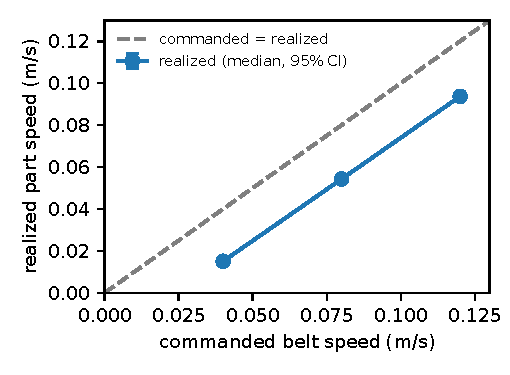
\includegraphics[width=\columnwidth]{fig_conv_speed.pdf}
\caption{Realized part speed versus commanded belt speed. The dashed line is the identity. The measured points lie on a line of slope one with a negative offset, not on a scaled identity.}
\label{fig:conv}
\end{figure}

\begin{figure}[t]
\centering
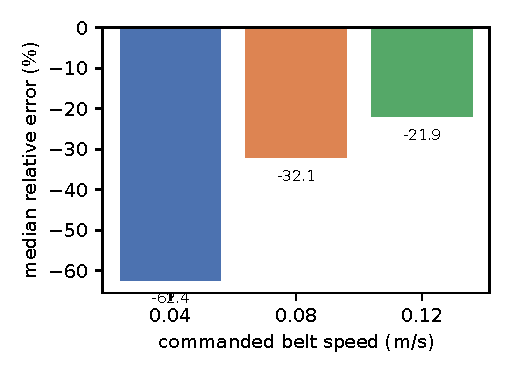
\includegraphics[width=\columnwidth]{fig_conv_error.pdf}
\caption{Median relative speed error by commanded speed. The error is largest at the lowest command because the absolute offset is approximately constant.}
\label{fig:converr}
\end{figure}

\subsection{The Direct Stop Works; the Safety-Agent Stop Does Not}
The emergency-stop experiment runs \estopN{} trials, half on each path, while the arm executes the same trajectory. The direct command path meets the stop criterion in \estopCommandSuccess\% of trials. The median signal-to-message latency is \estopCommandTzeroMs\,ms, the median time to a sustained low joint speed is \estopCommandTstopMs\,ms (95th percentile \estopCommandTstopTailMs\,ms), and the median post-signal overshoot is \estopCommandOvershootMed\,rad. The path publishes a \estopCommandJoints-joint trajectory with zero end velocities, and the controller accepts it; velocities are present in \estopCommandHasVel\% of the halt messages.

The safety-agent path meets the stop criterion in \estopSafetySuccess\% of trials. The agent publishes a four-joint halt with no velocities, and the controller rejects it because partial goals are disabled. The arm continues to its goal, with a median post-signal overshoot of \estopSafetyOvershootMed\,rad. The signal-to-message latency is short (\estopSafetyTzeroMs\,ms), so the failure is not a communication delay; it is a message-format mismatch. The halt message has \estopSafetyJoints{} joints, and velocities are present in \estopSafetyHasVel\% of trials.

This result fails the pre-registered safety-path criterion. It also explains the original sub-30\,ms claim: the original benchmark measured the latency of a loopback topic, not the arrest of an arm. The repaired measurement separates the two quantities and shows that the safety path does not arrest the arm at all. The direct path is a valid stop, but it is not the safety agent. As a sensitivity check at a more permissive 0.05\,rad/s threshold, the command path succeeds in \estopCommandSuccessSensitivity\% and stops in \estopCommandTstopSensitivityMs\,ms, while the safety path succeeds in \estopSafetySuccessSensitivity\%; the conclusion is unchanged.

\begin{figure}[t]
\centering
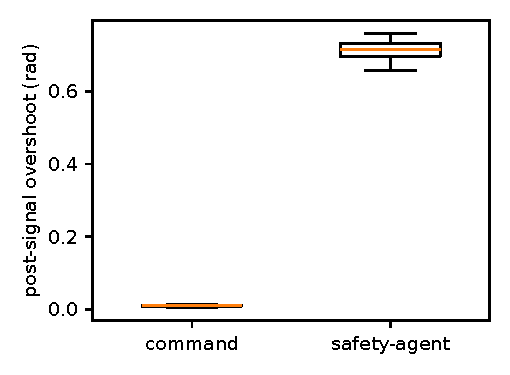
\includegraphics[width=\columnwidth]{fig_estop_overshoot.pdf}
\caption{Post-signal overshoot by stop path. The safety-agent path overshoots by nearly a radian because the controller rejects its partial, velocity-free halt.}
\label{fig:estop}
\end{figure}

\subsection{Kinematic Pre-Verification Filters Failures but Does Not Improve Intention-to-Treat Success}
The pre-verification experiment evaluates \nFourN{} planned targets with two pipelines. The baseline trusts the solver's success flag and executes the returned joints; it succeeds in \nFourBaselineSuccessPct\% of targets (Wilson 95\% CI [\nFourBaselineLoPct, \nFourBaselineHiPct]) and fails in \nFourBaselineExecFailPct\%. In this sample every baseline failure is a solver failure: the success flag is false, not a false positive, and the false-success rate is \nFourFalseSuccessPct\%. The N4 pipeline checks the forward-kinematics residual and the joint-limit margin, replans locally when the check fails, and rejects the plan if no candidate verifies. It executes \nFourCoveragePct\% of targets and succeeds in \nFourSuccessPct\% (CI [\nFourNFourLoPct, \nFourNFourHiPct]); among the plans it executes, the failure rate is \nFourExecFailPct\%.

The paired transitions explain the difference. N4 solves \nFourOnly{} target that the baseline fails, loses \nFourBaselineOnly{} targets that the baseline solves, solves \nFourBothSuccess{} with both pipelines, and solves \nFourNeither{} with neither. The paired risk difference in intention-to-treat success is \nFourRiskDiffPct{} percentage points (95\% CI [\nFourRiskDiffLoPct, \nFourRiskDiffHiPct]), with \nFourP. The gate therefore lowers the execution-failure rate among accepted plans, but that conditional comparison is not an intention-to-treat improvement: it removes failures by rejecting most of the targets that would have failed, and it also rejects \nFourBaselineOnly{} solvable targets while rescuing only \nFourOnly{}. We do not claim that the pre-registered criterion is met, because the accepted set is selected after verification and the pre-registered paired test was defined on the full target set.

The pre-registration specified a Newcombe interval for the risk difference; because the two pipelines share the same targets, we report a paired percentile bootstrap and record the change in the deviation log. The gate executes \nFourCoveragePct\% of targets and uses \nFourReplansMean{} replans per target on average. A stricter gate is not a free improvement; it trades coverage for a guarantee that the executed plans are verified.

\begin{figure}[t]
\centering
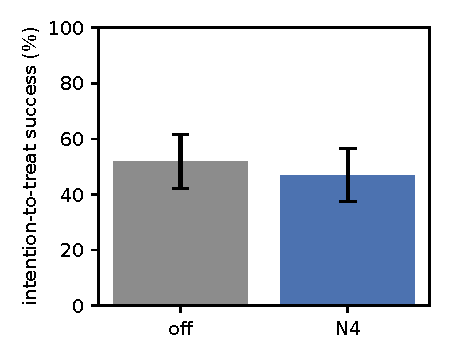
\includegraphics[width=\columnwidth]{fig_n4_success.pdf}
\caption{Intention-to-treat success with and without kinematic pre-verification. Error bars are Wilson 95\% intervals. The gate does not improve success on this target distribution.}
\label{fig:n4}
\end{figure}

\subsection{A 2.0\,s Watchdog Fires on Slow Calls and Not on Fast Ones}
The watchdog experiment runs \wdN{} language-model calls, \wdFastN{} fast and \wdSlowN{} slow, with the pre-registered \wdTimeoutS\,s timeout. The watchdog produces \wdFalsePosPct\% false positives on the fast calls and misses \wdMissedPct\% of the slow calls. On the slow calls the median detection latency is \wdMedianS\,s and the 95th percentile is \wdP95S\,s, which is \wdExcessP95S\,s above the timeout and inside the pre-registered one-polling-period allowance. The pre-registered H0f criterion is met. The watchdog was also exercised against a real Ollama call, which returned in \wdOllamaCallS\,s and did not fire.

\subsection{Kinematics-Anchored Depth Calibration Beats the Fixed Prior but Not the One-Point Baseline}
The depth experiment evaluates \nOneN{} held-out frames with \nOneRows{} method-by-frame rows. The calibration form is \nOneForm. The mean depth RMSE is \nOneNOneMeanMm\,mm for N1 (95\% CI [\nOneNOneLoMm, \nOneNOneHiMm]), \nOneFixedMeanMm\,mm for the fixed prior (CI [\nOneFixedLoMm, \nOneFixedHiMm]), \nOneOnePointMeanMm\,mm for the one-point anchor (CI [\nOneOnePointLoMm, \nOneOnePointHiMm]), and \nOneTwoPointMeanMm\,mm for the two-point fit (CI [\nOneTwoPointLoMm, \nOneTwoPointHiMm]). The two-point fit is unstable: its maximum per-frame RMSE is \nOneTwoPointMaxMm\,mm, against \nOneNOneMaxMm\,mm for N1.

The paired differences are the pre-registered test. N1 improves on the fixed prior by \nOneMinusFixedMm\,mm (CI [\nOneMinusFixedLoMm, \nOneMinusFixedHiMm]), winning on \nOneMinusFixedWins{} of \nOneN{} frames, so that interval excludes zero. N1 improves on the two-point fit by \nOneMinusTwoPointMm\,mm (CI [\nOneMinusTwoPointLoMm, \nOneMinusTwoPointHiMm]), winning \nOneMinusTwoPointWins{} frames. N1 does not, however, separate from the simple one-point anchor: the paired difference is \nOneMinusOnePointMm\,mm (CI [\nOneMinusOnePointLoMm, \nOneMinusOnePointHiMm]), winning \nOneMinusOnePointWins{} frames, and the interval includes zero. The pre-registered H2-N1 required N1 to beat both baselines; it therefore does not pass in full. The honest reading is that the kinematic anchor removes the fixed prior's bias and stabilizes the two-point fit, but the extra machinery does not buy a measurable improvement over a single well-placed anchor on this dataset.

\subsection{Scene Match Dominates and the Language-Model Confidence Collapses to Zero Weight}
The ambiguity experiment resolves \nThreeN{} prompts. The resolution-correct rate is \nThreeSuccessPct\% (\nThreeSuccessN{} of \nThreeN) and the parse rate is \nThreeParsePct\%. On the held-out test prompts (\nThreeTestN), the rate is \nThreeTestSuccessPct\% (\nThreeTestSuccessN{} of \nThreeTestN). The test AUROC is \nThreeSceneAuroc{} for the scene-match score (95\% CI [\nThreeSceneLo, \nThreeSceneHi]), \nThreeLlmAuroc{} for the calibrated language-model confidence (CI [\nThreeLlmLo, \nThreeLlmHi]), and \nThreeFusedAuroc{} for the fused score (CI [\nThreeFusedLo, \nThreeFusedHi]). The fusion weight fitted on the calibration split is \nThreeFusionWeight, so the fused score is the scene score. The paired AUROC difference against the language-model-only score is \nThreeFusedMinusLlmAuroc{} (CI [\nThreeFusedMinusLlmLo, \nThreeFusedMinusLlmHi]), and the interval includes zero. The pre-registered H2-N3 criterion is therefore not met. The fitted Platt slope is \nThreePlattA{} and the intercept is \nThreePlattB, which is close to a constant map: on this prompt set the model's verbal confidence carries little usable signal, and the scene match carries the discrimination.

\subsection{The Detector Generalizes to Held-Out Scenes, but the Requested Frame Count Is Not Met}
The detector experiment trains YOLOv8n at \detImgsz\,px for \detEpochs{} epochs on \detTrainN{} auto-labelled frames from scenes 1--20, validates on \detValN{} frames from scenes 21--24, and tests on \detTestN{} frames from scenes 25--30. The test mAP50 is \detMapFiftyTest{} and the test mAP50-95 is \detMapFiftyToNinetyFiveTest; the validation mAP50 is \detMapFiftyVal{} and the validation mAP50-95 is \detMapFiftyToNinetyFiveVal. At the fixed operating point (confidence 0.25, IoU 0.5) the test precision is \detOpPrecision{}, recall is \detOpRecall{}, and F1 is \detOpFOne, from \detOpTP{} true positives, \detOpFP{} false positives, and \detOpFN{} false negatives over \detTestN{} frames. The checkpoint is committed and its hash is in the ledger.

The experiment does not meet the original Phase~0f request of \detRequestedN{} frames. It produces \detTotalN{} frames (\detTrainN{} train, \detValN{} validation, \detTestN{} test), the reduced count declared in the pre-registration. The dataset is single-class, single-file, and rendered in one workcell, so the mAP should be read as a check that the labelling and training pipeline is sound, not as evidence that the detector transfers to a new cell, a new camera, or a cluttered bin. The 5,000-frame shortfall is reported rather than filled by repeating frames.

\begin{table}[t]
\centering
\caption{Pre-registered experiments and outcomes. Values are generated from the raw logs; see the ledger for sample sizes and intervals.}
\label{tab:results}
\setlength{\tabcolsep}{3pt}
\scriptsize
\begin{tabular}{@{}lll@{}}
\toprule
Experiment & Primary quantity & Outcome \\
\midrule
P0-REACH & recall at 5\,mm & \reachRecallCurrentPct\% current, \reachRecallOldPct\% historical \\
P0-CONV & realized/commanded ratio & \convRelErrA\%, \convRelErrB\%, \convRelErrC\% error \\
P0-ESTOP & halt success & \estopCommandSuccess\% command, \estopSafetySuccess\% safety \\
P0-WD & watchdog p95 latency & \wdP95S\,s, \wdFalsePosPct\% false positives \\
P2-N1 & depth RMSE & N1 \nOneNOneMeanMm\,mm, fixed \nOneFixedMeanMm\,mm \\
P2-N3 & test AUROC & scene \nThreeSceneAuroc, LLM \nThreeLlmAuroc, fused \nThreeFusedAuroc \\
P2-N4 & ITT success & \nFourBaselineSuccessPct\% off, \nFourSuccessPct\% on \\
P0-DET & mAP50 / mAP50-95 & test \detMapFiftyTest{} / \detMapFiftyToNinetyFiveTest \\
\bottomrule
\end{tabular}
\end{table}

\section{Negative Results, Non-Executed Phases, and Threats to Validity}
\label{sec:negative}
Five of the eight experiments return a negative or conditional result. The conveyor hypothesis fails because the plant does not realize the command. The safety-path hypothesis fails because the halt message is rejected. The pre-verification hypothesis is not supported as an intention-to-treat improvement: the gate removes execution failures from the plans it accepts, but it rejects more than half of the targets and lowers intention-to-treat success, so no practical improvement is claimed. N1 beats the fixed prior and the unstable two-point fit, but not the one-point anchor, so the pre-registered H2-N1 is only partly met. N3 fails because the fused score collapses to the scene score and the language-model confidence adds no discrimination. The reachability, watchdog, and detector hypotheses are supported, but each support is narrower than the original claim: the reachability gain is a model correction, the watchdog result is a timing check on a single local model, and the detector result is a single-class, single-file dataset.

Several phases could not be executed. N2 requires the pre-registered 50\,mm pick-and-lift predicate, and the position-controlled jaws cannot satisfy it: the first contact step applies 9--10\,N, shoves the 45\,g cube 1--7\,mm, and the cube escapes during the lift. The best observed lift was 0.9\,mm. The conveyor plugin also pinned the workpieces to the deck by zeroing their vertical and angular velocities every tick; that platform defect is repaired, but the gripper defect remains. Phase~3 learned policies require T1 demonstrations, and T1 is not executable. Human inter-annotator agreement requires independent annotators, and none are available; a second language model is not a human substitute. Hardware trials require a robot and a serial device, and neither is present. The original 5,000-frame detector request is reduced by the pre-registration to 1,000 training frames (1,240 total), and that shortfall is reported rather than filled by repeating frames.

The N2 decision is recorded as not executed, not simulated and not re-labelled with a weaker predicate. The same rule applies to every T1-dependent experiment (the T1 cell of the suite, the grasp and ablation studies, and the learned-policy demonstrations). Each cell is recorded in the audit with its blocking condition, rather than filled with an estimate.

The threats to validity are specific. The conveyor plant is kinematic, so the measured offset may be an artifact of the velocity-write path rather than a friction property. The arm is a four-degree-of-freedom mechanism with a small reachable region, so the pre-verification result may not transfer to a six-degree-of-freedom arm with a larger workspace. The emergency-stop result depends on the controller configuration; a controller that accepts partial goals would not reject the safety halt. The trial counts are sufficient for the large effects reported here but not for small ones, and the pre-registration labels the smaller cells as exploratory.

The audit itself has a limitation: it was performed by the same group that built the stack. We mitigated this by freezing the protocol before evaluation, by using only executed code and raw logs, and by reporting failures. We did not have an independent auditor. An external audit would be stronger, and we recommend it for any claim that is used to justify a deployment.

\section{Conclusion}
\label{sec:conclusion}
We audited a modular manipulation stack, repaired its instrumentation, pre-registered four questions, and re-measured them from clean commits. The reachability result is reproducible and the historical gap is explained by a solver revision. The conveyor does not realize its command; it realizes the command minus a nearly constant offset, while the visual belt is stationary and the rollers spin implausibly fast. The direct emergency stop works, but the safety-agent stop is rejected by the controller and the arm continues to its goal. A kinematic pre-verification gate removes execution failures from the plans it accepts, but it rejects more than half of the targets and does not improve intention-to-treat success on the sampled workspace.

The broader lesson is that a benchmark is a measurement chain, and every link must be checked. A topic can have several publishers; a service can be a loopback; a transform can be a placeholder; a solver can report success for a pose it did not reach; a controller can reject a goal without an error. None of these failures is exotic. Each produces a number that looks like evidence. Pre-registration and provenance do not prevent the failures, but they make them visible, and visibility is the precondition for repair.

\section*{Data Availability}
The pre-registration, the audit, the experiment scripts, the raw per-trial logs, the number generator, the macro file, and the ledger are in the repository. The raw logs are also packaged as \texttt{data/journal/raw\_logs.tar.gz} because the live log directory is git-ignored. The paper is compiled from the macro file; no outcome number is typed into the manuscript.

\section*{Acknowledgment}
The authors thank the maintainers of ROS~2, Gazebo, and the open-source robotics stack on which this work depends.

\bibliographystyle{IEEEtran}
\bibliography{references}

\end{document}
